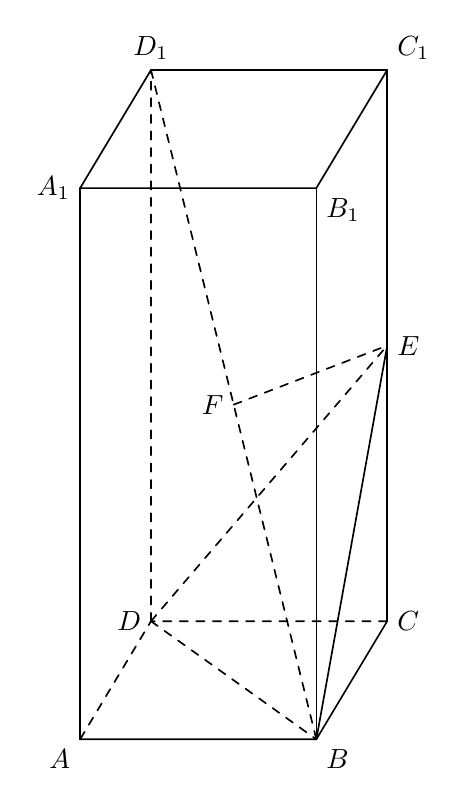
\begin{tikzpicture}[line width=0.6pt, line join=round, line cap=round]
  \coordinate (A) at (0,0);
  \coordinate (B) at (3,0);
  \coordinate (D) at (0.9,1.5);
  \coordinate (C) at (3.9,1.5);
  \coordinate (A1) at (0,7);
  \coordinate (B1) at (3,7);
  \coordinate (D1) at (0.9,8.5);
  \coordinate (C1) at (3.9,8.5);
  \coordinate (E) at (3.9,5);
  \coordinate (F) at (1.95,4.25);
  % bottom / top
  \draw (A) -- (B) -- (C);
  \draw[dashed] (C) -- (D) -- (A);
  \draw (A1) -- (B1) -- (C1) -- (D1) -- cycle;
  % verticals
  \draw (A) -- (A1);
  \draw (B) -- (B1);
  \draw (C) -- (E) -- (C1);
  \draw[dashed] (D) -- (D1);
  % face / body diagonals
  \draw[dashed] (D1) -- (B);
  \draw[dashed] (D) -- (B);
  \draw[dashed] (D) -- (E);
  \draw[dashed] (F) -- (E);
  \draw (E) -- (B);
  % labels
  \node[below left] at (A) {$A$};
  \node[below right] at (B) {$B$};
  \node[left] at (D) {$D$};
  \node[right] at (C) {$C$};
  \node[left] at (A1) {$A_{1}$};
  \node[below right] at (B1) {$B_{1}$};
  \node[above] at (D1) {$D_{1}$};
  \node[above right] at (C1) {$C_{1}$};
  \node[right] at (E) {$E$};
  \node[left] at (F) {$F$};
\end{tikzpicture}
